\subsection{SWOT-Analyse} \label{swot}
Um nun externe und interne Informationsbereiche miteinander zu verbinden, wird die \as SWOT-Analyse\adl genutzt. Mit
dieser Betrachtung ist es möglich, die Stärken und Schwächen des Unternehmens kombiniert mit den Chancen und Risiken der
Mikro- und Makroumwelt zu untersuchen und Strategien abzuleiten. (Vgl. \cite{Brun2014} S.\,43)

\noindent Dabei wurden zum Praxisbeispiel „RinnenRobo“ die folgenden Chancen erarbeitet:

    \begin{itemize}
        \item \textbf Demographischer Wandel
        
            Da das Produkt \as RinnenRobo\adl den Menschen das Säubern ihrer Dachrinnen erleichtert und auch sicherer
            gestaltet, ist es besonders für ältere Menschen interessant. Diese können möglicherweise auf Grund von
            körperlichen Einschränkungen nicht mehr per Hand die Dachrinnen reinigen. Somit vergrößert der
            demographische Wandel die Gruppe der potenziellen Abnehmer in diesem Bereich.
        \item \textbf Technologische Trends
            
            Das Produkt \as RinnenRobo\adl könnte außerdem großes Interesse bei technisch-interessierten Menschen
            wecken. Auch die Größe dieser Gruppe könnte durch den Trend zur Digitalisierung und Technologisierung
            wachsen.
        \item \textbf Förderung von Innovation
        
            Da es nur ein Produkt gibt, welches in ähnlicher Weise zum \as RinnenRobo\adl funktioniert, wäre es denkbar,
            eine finanzielle Förderung zur Entwicklung des Roboters einzustreichen. Diese Förderung könnte dabei
            entweder staatlicher oder privater Natur sein.
    \end{itemize}

\noindent Nachdem nun die Chancen betrachtet wurden, sollen im Folgenden die Risiken näher betrachtet werden:

    \begin{itemize}
        \item Weniger Eigenheime

            In Deutschland gibt es momentan einen sinkenden Anteil an Eigenheimen und einen dadurch bedingten, höheren
            Anteil an Mietwohnungen und -häusern (Vgl. \cite{Mueller2021}). Dieser Umstand könnte dazu führen, dass
            weniger \as RinnenRobos\adl verkauft werden, da davon ausgegangen werden kann, dass Privatpersonen mit 
            Eigenheim mehr Wert auf dessen Gepflegtheit legen als Personen ohne Eigenheim.

        \item Steigende Produktionskosten
        
            Durch höhere Rohstoff- und Logistikkosten werden die Produktionskosten momentan stark erhöht. Diese
            Preiserhöhung muss im Endverkaufspreis an den Kunden weitergegeben werden. Auf Grund dieser Preissteigerung
            könnten sich einige potenzielle Käufer doch gegen den Erwerb eines \as RinnenRobos\adl entscheiden.
    \end{itemize}

\noindent Nachdem der externe Informationsbereich nun betrachtet wurde, ist nachfolgend der interne Informationsbereich
zu untersuchen. Begonnen wird mit den Stärken des Unternehmens:

    \begin{itemize}
        \item Arbeitserleichterung und Zeitersparnis
        
            Durch das Produkt \as RinnenRobos\adl sparen sich Käufer viel Zeit bei der Reinigung ihrer Dachrinnen.
            Außerdem ist die Arbeit auch körperlich stark erleichtert. Diese Vorteile könnte das Unternehmen zur
            Gewinnung neuer Kunden nutzen.

        \item Erhöhte Sicherheit
        
            Auch führt die Benutzung des \as RinnenRobos\adl zu einer höheren Sicherheit beim Säubern der Dachrinnen.
            Auch dies ist ein weiteres Verkaufsargument für das Unternehmen.
    \end{itemize}

\noindent Schlussendlich werden nun noch die Schwächen des Unternehmens betrachtet:

    \begin{itemize}
        \item Wartung und Instandhaltung

            Da der \as RinnenRobos\adl ein technisches Gerät ist, kann man davon ausgehen, dass es aufwendiger ist,
            diesen Instand zu halten, als einen Besen, den man sonst zur Säuberung der Dachrinnen verwenden würde.
            Dieser Umstand könnte einige potenzielle Kunden vom Kauf abhalten.
        \item Höherer Preis
        
            Auch der Preis ist, verglichen zum klassischen Besen, um einiges höher. Auch dies könnte für die
            Interessenten ein Grund sein, den \as RinnenRobos\adl nicht zu erwerben.
    \end{itemize}

\noindent Nachdem nun sowohl externe als auch interne Informationsbereiche betrachtet wurden, ist es möglich, diese in
eine SWOT-Matrix zu bringen. Aus dieser Matrix kann man dann die verschiedenen Strategien konzipieren. Die graphische
Darstellung in Tabellenform ist die folgende:

    \begin{figure}[ht]
        \centering
        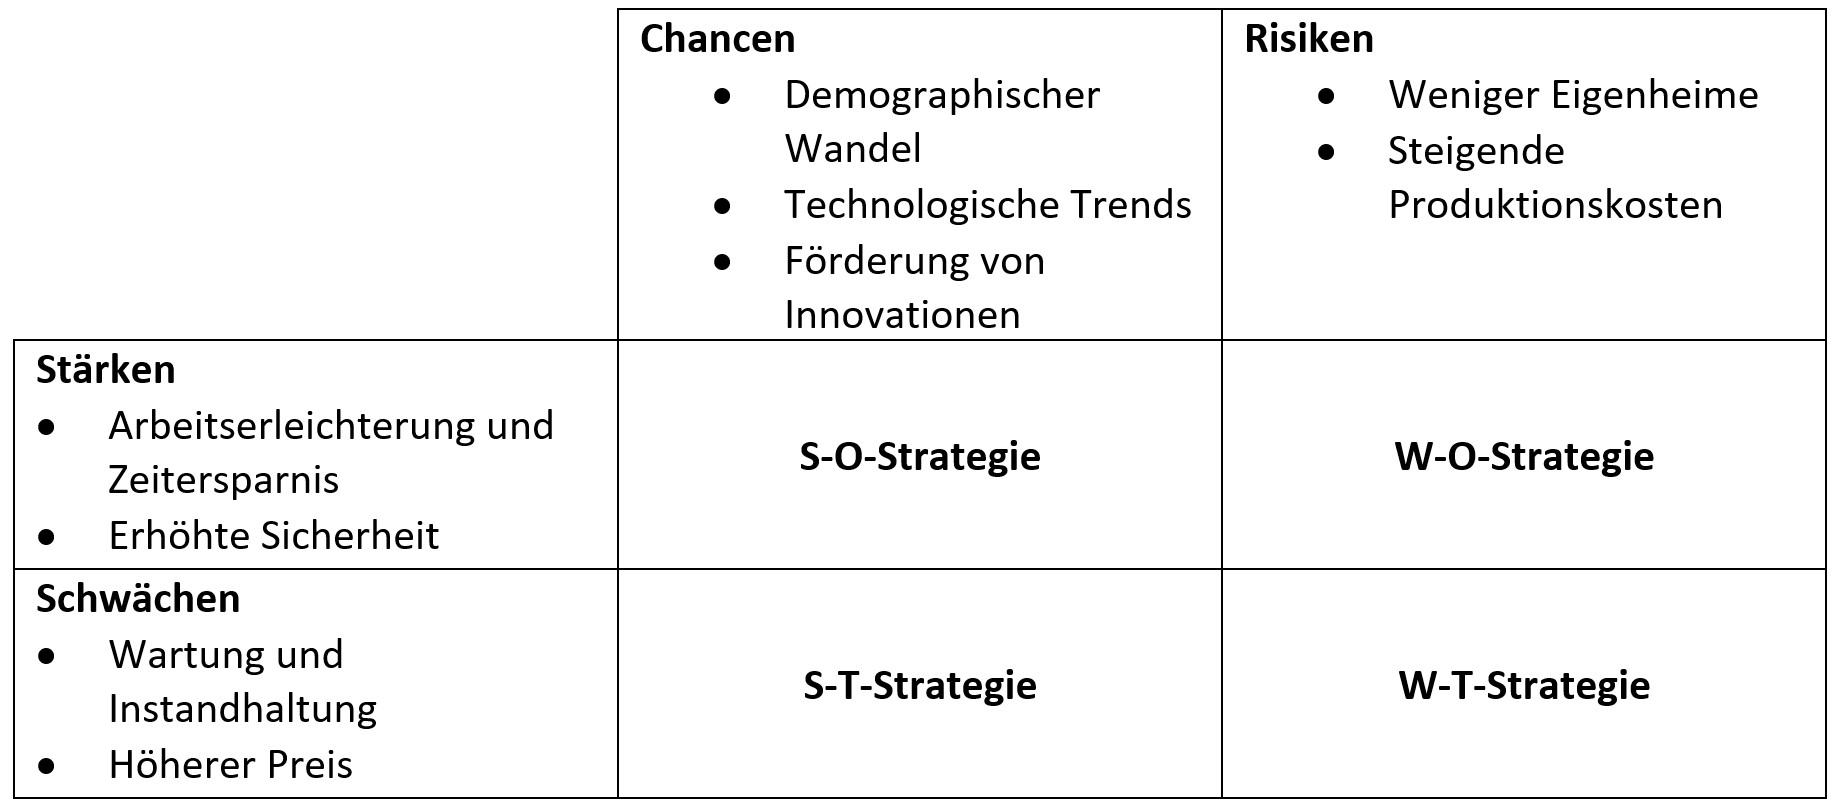
\includegraphics[width = 0.9\textwidth]{Eigene Darstellungen/SWOT Tabelle.jpg}
    \end{figure}

\noindent Nun müssen aus dieser Tabelle verschiedene Strategien abgeleitet werden. Diese Strategien finden sich in den
vier Zellen, in denen sich interne und externe Informationsbereiche überschneiden.

\noindent Für den \as RinnenRobos\adl wurden die folgenden Strategien formuliert:

    \begin{itemize}
        \item S-O-Strategie (Chancen und Stärken)
        
            Hier wäre es denkbar, das technologische Interesse der potenziellen Kunden durch eine Bedienung per App
            anzusprechen.

            Außerdem wäre es im Hinblick auf den demographischen Wandel sinnvoll, mit erhöhter Sicherheit und
            körperlicher Entlastung zu werben, um ältere Zielgruppen anzusprechen.

        \item W-O-Strategie (Chancen und Schwächen)
        
            Hier wäre es denkbar, einen Reparaturdienst auch über die Garantie hinaus anzubieten. Somit würde man den
            Kunden die Aufgabe der Wartung und Instandhaltung erleichtern und zusätzliche Einnahmen generieren.
            
            Möglich wäre es vermutlich außerdem die höheren Produktionskosten durch staatliche oder private Fördergelder
            auszugleichen, um auch den Endverkaufspreis attraktiver für den Kunden zu machen.        

        \item S-T-Strategie (Risiken und Stärken)
        
            Um die Umsatzeinbußen aus dem sinkenden Anteil von Eigenheimen auszugleichen, wäre es denkbar den 
            \as RinnenRobos\adl auch an Unternehmen zu vertreiben. Hier stehen besonders Hausmeister und entsprechende
            Gebäudepfleger im Fokus, da man durch diese auch Umsatz mit dem Einsatz an Mehrparteienhäusern generieren
            könnte. Bei dieser Kundengruppe könnte man besonders mit der Arbeitserleichterung und Zeitersparnis, die die
            Benutzung des \as RinnenRobos\adl den Kunden bringt, werben.

        \item W-T-Strategie (Risiken und Schwächen)
        
            Hier wäre es möglich eine günstigere Version des \as RinnenRobos\adl, eine Modellreihe mit weniger
            Funktionen, zu veröffentlichen, um auch kapitalschwächere Kundengruppen zu erreichen.
            
            Außerdem wäre es denkbar einen Mietservice für die Roboter anzubieten, um dem Kunden die Anschaffungskosten
            und die Wartung zu ersparen. 
        
    \end{itemize}